\chapter{Introduction}\label{sec:intro}

\paragraph{Presentation:}FA$\mu$ST is a C++ toolbox, useful to decompose a given dense matrix into a product of sparse matrices in order to reduce its computational complexity (both for storage and manipulation). In Figure \ref{fig:presentation}, the matrix \textbf{A} represents the dense matrix and $\mathbf{S_j}$ correspond to the sparse matrices as $\mathbf{A}=\prod_{j=1}^J\mathbf{S_j}$.

\begin{figure}[!h] %%[!htbp]
\centering
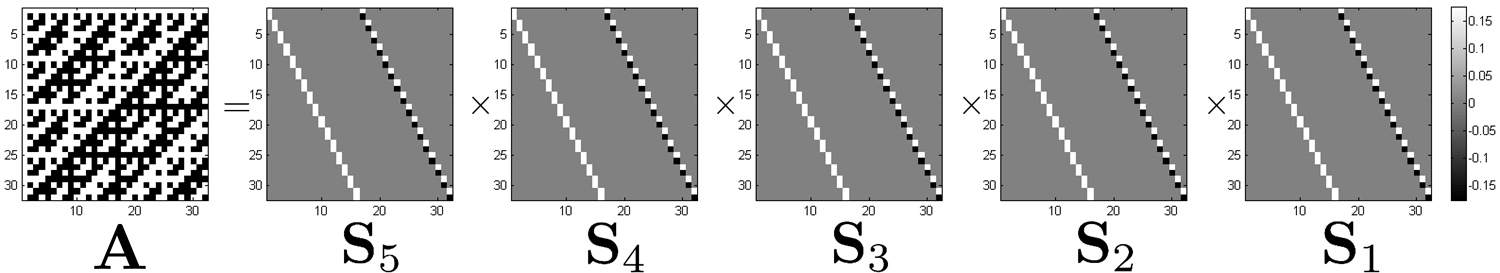
\includegraphics[scale=0.5]{images/hadamard32_bw.pdf}
\caption{presentation}
\label{fig:presentation}
\end{figure}

FA$\mu$ST can be used to speed up iterative algorithms commonly used for solving high dimensional linear inverse problems. The algorithms implemented in the toolbox are described in details by Le Magoarou.\cite{LeMagoarou2016}.
The FA$\mu$ST toolbox is delivered with a Matlab wrapper. 
For more information on the FAuST Project, please visit the website of the project: \url{http://faust.gforge.inria.fr}.

%\paragraph{Brief description:} 
%$A=\prod_{j=1}^J S_j$.


\paragraph{License:}Copyright (2016) Luc Le Magoarou, Remi Gribonval INRIA Rennes, FRANCE \\
The FAuST Toolbox is distributed under the terms of the GNU Affero General Public License. This program is free software: you can redistribute it and/or modify it under the terms of the GNU Affero General Public License as published by the Free Software Foundation. This program is distributed in the hope that it will be useful, but WITHOUT ANY WARRANTY; without even the implied warranty of MERCHANTABILITY or FITNESS FOR A PARTICULAR PURPOSE.  See the GNU Affero General Public License for more details. You should have received a copy of the GNU Affero General Public License along with this program.  If not, see \url{http://www.gnu.org/licenses/}.


\paragraph{Organization:}Chapter \ref{sec:InstallUnix} explains how to install the library FA$\mu$ST for UNIX platform and Chapter \ref{sec:WinInstall} corresponds to the Windows installation. Chapter \ref{sec:firstUse} shows quickly how to use this library and finally an example is given Chapter \ref{sec:example}. 